\begin{frame}{Scalability - Communication graph}
    Minimum information required to determine the solution of a single traffic light $\bar{u}_i$
    \begin{center}
    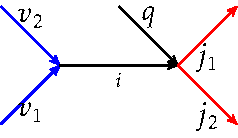
\includegraphics[scale=0.7]{fig_66_connectivityGraph}
    \end{center}
    Set of roads that can "talk" to $i$:
    \[
    \mathcal{S}_i = \neighUp_i\cup\neighDown_i\cup\mathcal{I}_i,
    \]
    %
    where
    %
    \[
    \mathcal{I}_i = \{q: \neighDown_q \equiv \neighDown_i\}.
    \]
    
    \metroset{block=fill}
    \begin{block}{Why?}
    $\neighUp_i$ and $\neighDown_i$ are needed for density prediction.
    $\mathcal{I}_i$ is needed for constraints over traffic lights.
    \end{block}
\end{frame}